\documentclass{article}
\usepackage{amsmath}
\usepackage{verbatim}
\usepackage[margin=1in]{geometry}
\setlength\parindent{0pt}
\usepackage{color}
\usepackage{graphicx}
\usepackage{hyperref}
% \usepackage{subcaption}
%\usepackage{tabularx}
%\usepackage{float}

\begin{document}


\begin{center}
\Huge{\textsc{Homework Five Report}} 

\Large\textsc{CMPS242 - Fall 2015}\\

\large{Andrei Ignat  \hfill Sabina Tomkins \hfill Guangyu Wang} 
\end{center}

%fix the title

\section{Intro}

\section{Data Preprocessing}

\subsection{Final data used for training}

\section{Environment}
We used python exclusively, and in particular we used scikit-learn for all classifiers. 



\subsection{Individual Classifiers}
Each of the following classifiers we tried on its own, and tried to tune the parameters for. When we combined classifiers we therefore used the best parameters found in the parameter tuning process. The classifiers we used are: Support Vector Machine, Logistic Regression, AdaBoost, Random Forest, Decision Trees, and K Nearest Neighbors. We chose these classifiers as they have been covered in class, \\

[insert a reason for each one why it may do ok on this dataset]  \\

Accuracy was used as the metric with which to compare classifiers. To see the results from the parameter tuning process please see the Appendix. Both in the parameter tuning, and in the final results below, we used 5-Fold cross validation. However in the ensemble we held out 40\% of the training set for validation.\\

\begin{tabular}{|c|c|c|c|c|c|c|}
\hline
& SVM & Decision Trees & KNN & Random Forest & Logistic Regression & AdaBoost   \\
\hline
Accuracy & SVM & Decision Trees & KNN & Random Forest & Logistic Regression & AdaBoost   \\

\hline
\end{tabular}\\

\subsection{Combined Classifiers}

\section{Results}

\section{Analysis}


\section{Appendix}
\graphicspath{../}

 \begin{figure}[h!]
 \centering
  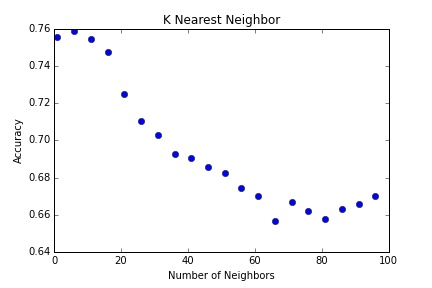
\includegraphics[width=0.5\textwidth]{NearestNeighbor.jpg}
 \caption{Tuning number of neighbors nearest neighbor}
 \end{figure}

 \begin{figure}[h!]
 \centering
  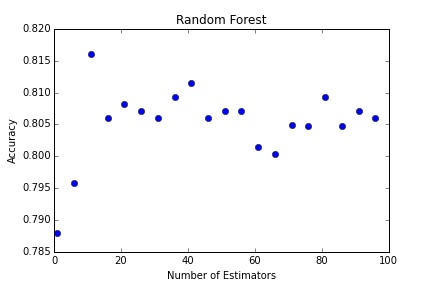
\includegraphics[width=0.5\textwidth]{RandomForest.jpg}
 \caption{Tuning number of estimators, Random Forest}
 \end{figure}
 
 


\bibliography{proposal_biblio}
\bibliographystyle{plain}

\end{document}
